\documentclass[titlepage, 12pt]{article}

% Packages
\usepackage[margin = 0.75in]{geometry}
\usepackage[hidelinks]{hyperref}
\usepackage{amsmath}
\usepackage{float}
\usepackage{graphicx}
%\usepackage{newtxtext}  % WHY IS THIS HERE
\usepackage{listings}
\usepackage{color}

% Default fixed font does not support bold face
\DeclareFixedFont{\ttb}{T1}{txtt}{bx}{n}{10} % for bold
\DeclareFixedFont{\ttm}{T1}{txtt}{m}{n}{10}

% Define colors
\definecolor{deepblue}{rgb}{0,0,0.5}
\definecolor{deepred}{rgb}{0.6,0,0}
\definecolor{deepgreen}{rgb}{0,0.5,0}


% Python style for highlighting
\newcommand\pythonstyle{\lstset{
    language=Python,
    basicstyle=\ttm,
    otherkeywords={self},             % Add keywords here
    keywordstyle=\ttb\color{deepblue},
    emph={bin,_prod,__name__},          % Custom highlighting
    emphstyle=\ttb\color{deepred},    % Custom highlighting style
    stringstyle=\color{deepgreen},
    commentstyle=\color{deepgreen},
    frame=tb,                         % Any extra options here
    showstringspaces=false            %
}}
\newcommand\pythonexternal[2][]{{\pythonstyle\lstinputlisting[#1]{#2}}}

\lstdefinestyle{data}
{
    basicstyle=\footnotesize\ttfamily,
    breaklines=true,
}

% Author information
\title{ENCM 467 Lab 1\\Static Behaviour of N and P channel MOS
transistors and a simple nMOS inverter}
\author{Andreas Smit}
\date{September 28, 2020}


% Settings
\setlength{\parindent}{0pt}

\begin{document}
    \maketitle

    \section{LT Spice MOSFET Operation}
    \subsection{Operation of a NMOS transistor in LT Spice}
    Figure \ref{fig:part_1a_circ} shows the NMOS circuit used to test.
    \begin{figure}
        \centering
        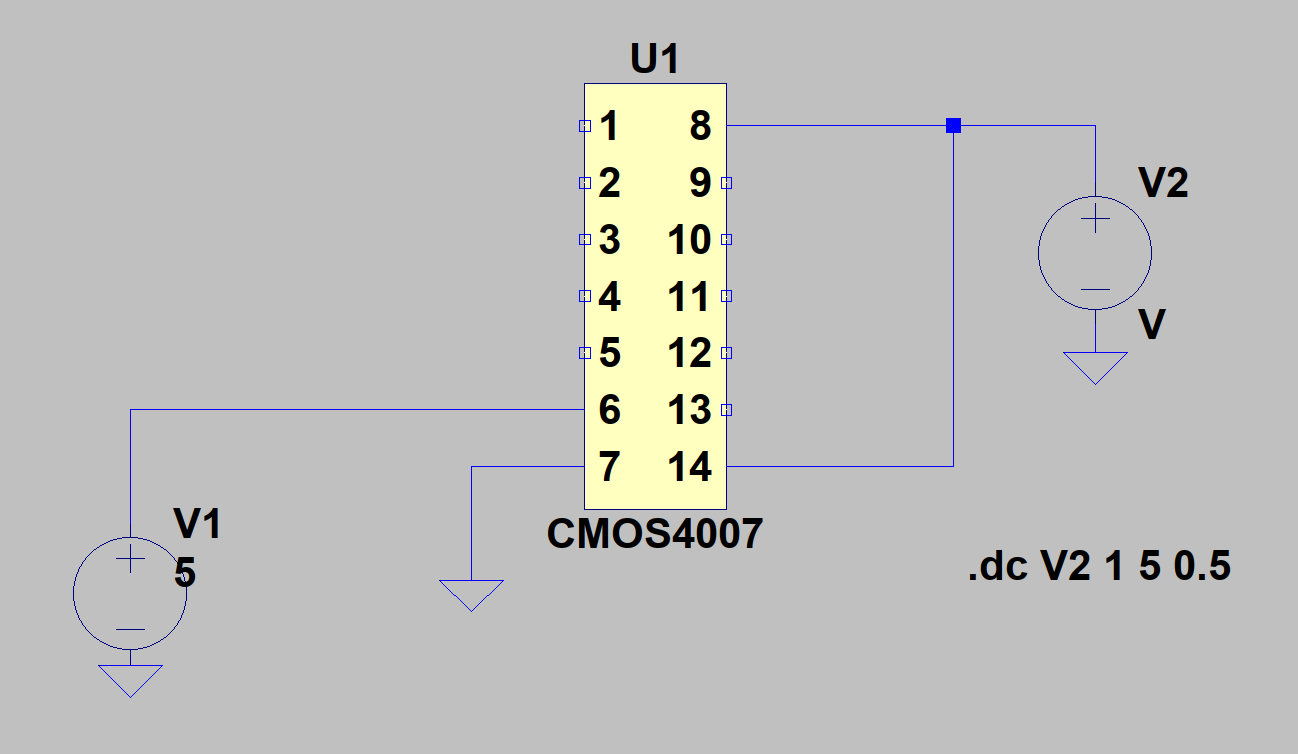
\includegraphics[width=0.7\textwidth]{figures/nmos_circuit.png}
        \caption{The NMOS circuit analyzed in LT Spice}
        \label{fig:part_1a_circ}
    \end{figure}
    Figure \ref{fig:part_1a_fig} shows the NMOS IV characteristics.
    \begin{figure}[H]
        \centering
        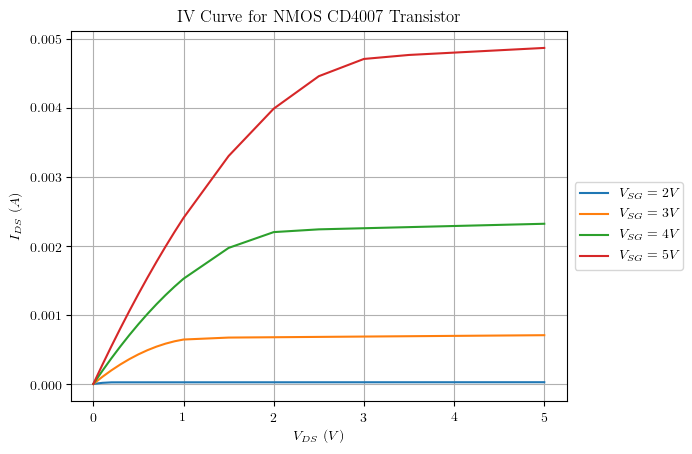
\includegraphics[width= 0.7\textwidth]{figures/part_1_nmos.png}
        \caption{Operating characteristics of the NMOS transistor. The
        raw data is in appendix \ref{sec:data}}
        \label{fig:part_1a_fig}
    \end{figure}

    \subsection{Operation of a PMOS transistor in LT Spice}
    Figure \ref{fig:part_1b_circ} shows the PMOS circuit used to test.
    \begin{figure}
        \centering
        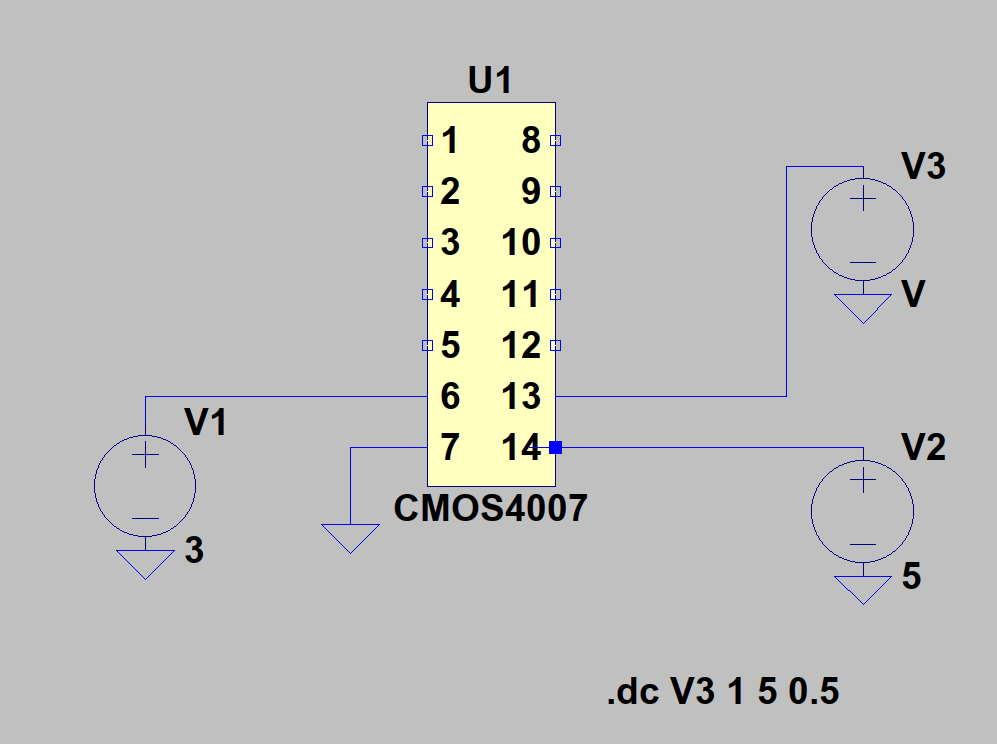
\includegraphics[width=0.7\textwidth]{figures/pmos_circuit.png}
        \caption{The PMOS circuit analysed in LT Spice}
        \label{fig:part_1b_circ}
    \end{figure}
    Figure \ref{fig:part_1b_fig} shows the PMOS IV characteristics.
    \begin{figure}[H]
        \centering
        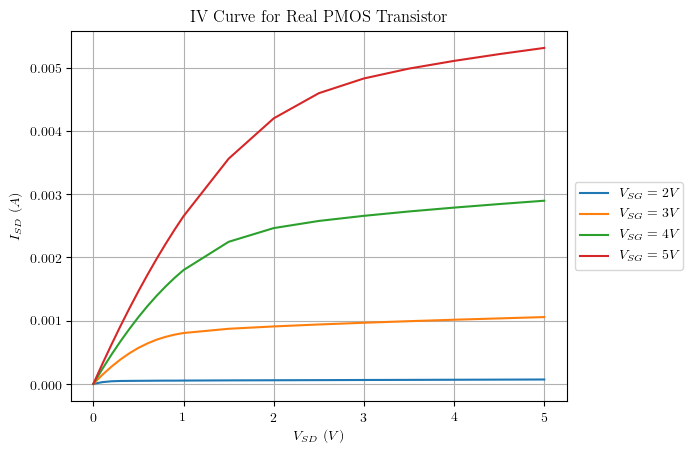
\includegraphics[width= 0.7\textwidth]{figures/part_3_pmos.png}
        \caption{Operating characteristics of the PMOS transistor. The
        raw data is in appendix \ref{sec:data}}
        \label{fig:part_1b_fig}
    \end{figure}


    \subsection{Analysis of the nMOS and pMOS circuits.}
    \label{sec:sim_sol1}
    The complete solution for the nMOS circuit will be shown, however
    the same method is used for the pMOS circuit and is very similar.
    \subsubsection{Solution of parameters for nMOS circuit}
    \label{sec:nmos_sol}
    We know that the current $I_D$ for a nMOS transistor in triode is
    given by
    \begin{equation}\label{eq:triode_eq}
        I_D = \frac{k_n}{2}\left(2(V_{GS} - V_T)V_{DS} - V_{DS}^2\right)
        (1 + \lambda V_{DS})
    \end{equation}
    Equation \eqref{eq:triode_eq} is cubic in terms of $V_{DS}$ and can
    be written as a third degree polynomial,
    \begin{equation}\label{eq:triode_poly}
        I_D = -\frac{1}{2}k_n\lambda V_{DS}^3
        + \left(k_n\lambda V_{sat} -\frac{k_n}{2}\right)V_{DS}^2
        + k_nV_{sat} V_{DS}
    \end{equation}
    where $V_{sat} = V_{GS} - V_T$. Fitting the data in for $V_{GS} =
    5V$ in figure \ref{fig:part_1a_fig} for $V_{DS} \leq 3V$ to a
    cubic equation gets us the graph in figure \ref{fig:part_1a_cube}
    which has an equation of the form
    \begin{equation}\label{eq:poly_fit}
        I_{D} = AV_{DS}^3 + BV_{DS}^2 + CV_{DS}
    \end{equation}
    \begin{figure}[H]
        \centering
        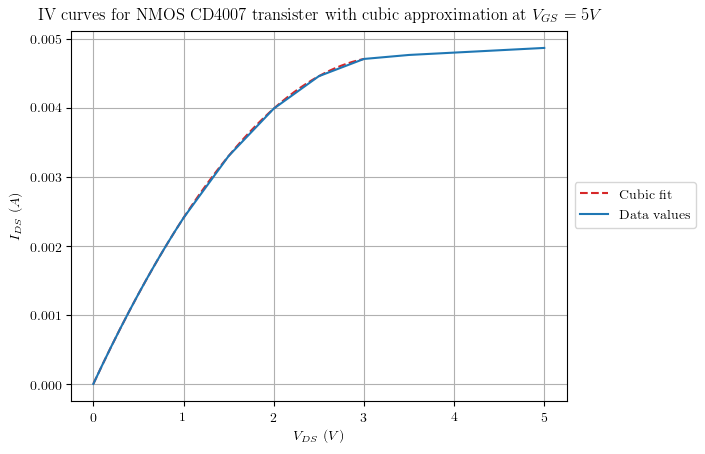
\includegraphics[width=0.75\textwidth]{figures/part_1_ncube.png}
        \caption{The IV curve for the nMOS transistor for $V_{GS} = 5V$.
            The cubic curve of best fit for $V_{DS} < 3V$ is plotted as
        well. Notice that they are a very good fit}
        \label{fig:part_1a_cube}
    \end{figure}
    The python code in appendix \ref{sec:code} is used to get the
    polynomial fit, and the constants $A$, $B$, and $C$.


    Relating the equations \eqref{eq:triode_poly} and
    \eqref{eq:poly_fit} the following system of non-linear equations is
    formed.
    \begin{equation}\label{eq:cases_from_hell}
        \begin{cases}
            A = -\frac{1}{2}k_n\lambda\\
            B = k_n\lambda V_{sat} - \frac{k_n}{2}\\
            C = k_n V_{sat}
        \end{cases}
    \end{equation}
    To solve equation \eqref{eq:cases_from_hell} for $k_n$, $\lambda$
    and $V_{sat}$ we must start by substituting $A$ and $C$ into $B$.
    \begin{align*}
        B &= k_n\lambda V_{sat} - \frac{k_n}{2}\\
        &= \frac{-2}{-2} k_n\lambda \frac{k_n}{k_n}V_{sat} -
        \frac{k_n}{2}\\
        &=-2\left(-\frac{1}{2}k_n\lambda\right)
        \frac{1}{k_n}(k_nV_{sat}) - \frac{k_n}{2}\\
        &= -\frac{2AC}{k_n} - \frac{k_n}{2}\\
        0 &= \frac{k_n^2}{2} + Bk_n + 2AC\\
        k_n &= -B \pm \sqrt{B^2 - 4AC}
    \end{align*}
    Using the value of $k_n$ determined above and the formulas for $A$
    and $C$ in equation \eqref{eq:cases_from_hell} we can determine all
    of the constants.

    The python script in appendix \ref{sec:code} gets values
    \texttt{A = -6.50707e-06}, \texttt{B = -3.91764e-04}, and \texttt{C
    = 2.80235e-03}, which can then be used to solve for the values of
    $k_n$, $\lambda$, and $V_{sat}$ as shown below.
    \begin{align*}
        k_n &= 867.6\mu A/V^2\\
        \lambda &= 0.015 V^{-1}\\
        V_T &= 1.77 V
    \end{align*}
    \subsubsection{Solution of parameters for a pMOS transistor}
    This will be done very similarly to the analysis shown in section
    \ref{sec:nmos_sol}. Using the same curve fitting approach the fit of
    the data onto a cubic polynomial is shown in figure
    \ref{fig:part_1b_cube}
    \begin{figure}[H]
        \centering
        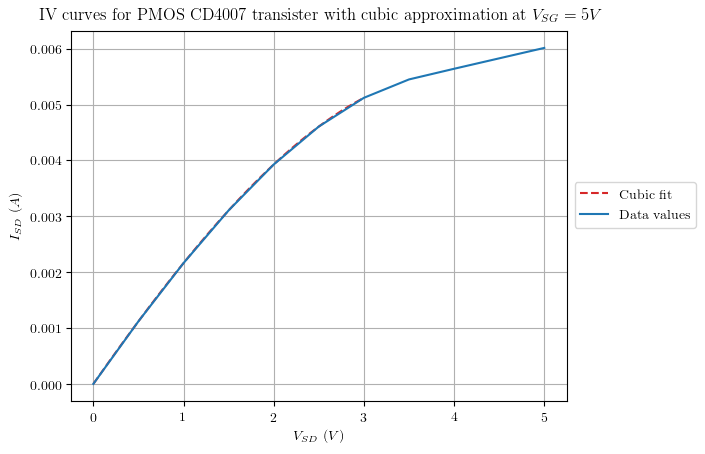
\includegraphics[width=0.75\textwidth]{figures/part_1_pcube.png}
        \caption{The IV curve for the pMOS transistor for $V_{SG} = 5V$
        The cubic curve of best fit for $V_SD < 3V$ is plotted as well.
        Notice that they are a good fit.}
        \label{fig:part_1b_cube}
    \end{figure}
    They python script gets values of \texttt{A = -2.88000e-=5},
    \texttt{B = -1.12640e-04} and \texttt{C = 2.30400e-03}, which can be
    used to find the constants,
    \begin{align*}
        k_p &= 640.0\mu A/V^2\\
        \lambda &= 0.09 V^{-1}\\
        V_T &= -1.4 V
    \end{align*}

    \subsection{Alternative Measurement Method for the threshold voltage}
    \label{sec:sim_sol2}
    Using the circuits in figure \ref{fig:part_1d_circ} with the left
    being an NMOS transistor and the right being a PMOS transistor we
    can find the curves shown in figures \ref{fig:part_1d_n} and
    \ref{fig:part_1d_p}
    \begin{figure}[H]
        \centering
        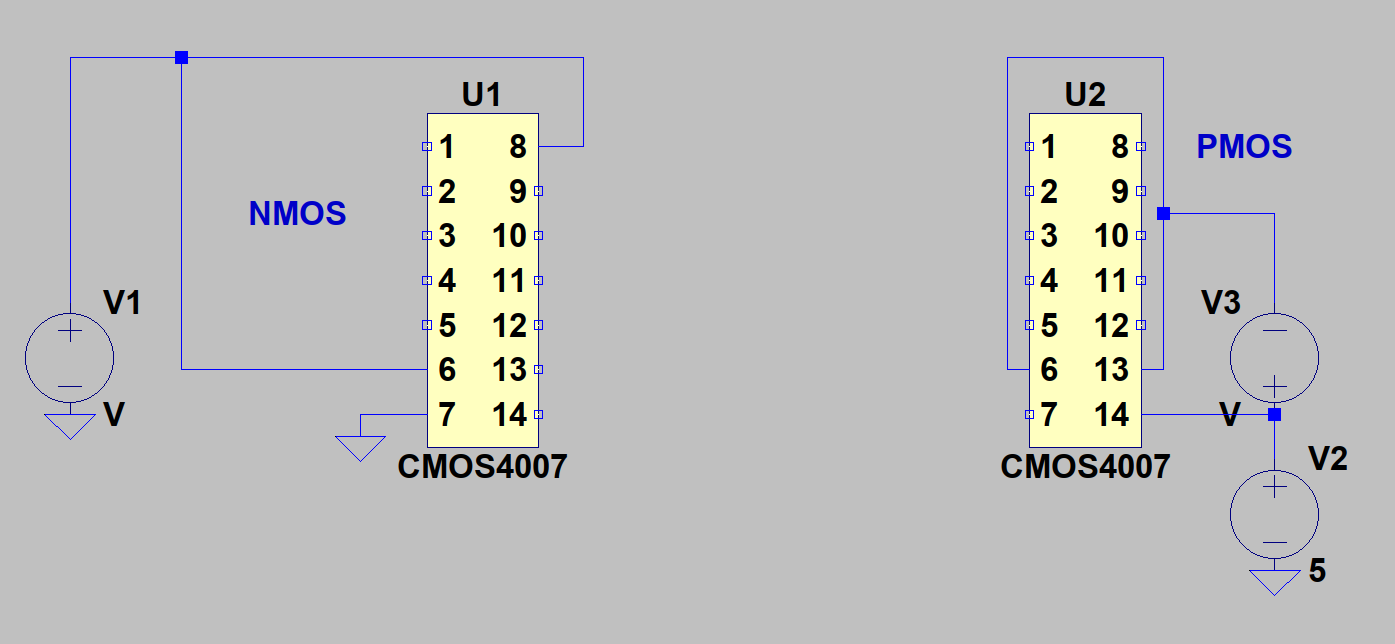
\includegraphics[width=0.7\textwidth]{figures/part1d_circuit.png}
        \caption{The NMOS and PMOS circuits used to measure the
        threshold voltage. Note that the circuit will enter saturation
        when it turns on.}
        \label{fig:part_1d_circ}
    \end{figure}
    \begin{figure}[H]
        \centering
        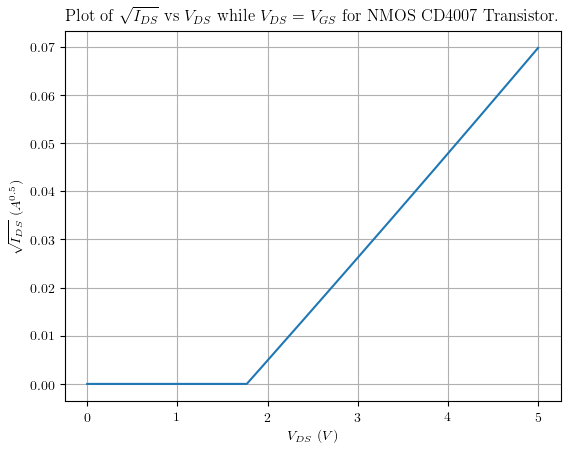
\includegraphics[width = 0.7\textwidth]{figures/part_1_nsqrt.png}
        \caption{The graph of $\sqrt{I_{DS}}$ vs $V_{DS}$ for the NMOS
        transistor. It can be seen from the graph that the cut-in
        voltage is the corner at $V_{DS} = 1.77V$.}
        \label{fig:part_1d_n}
    \end{figure}
    \begin{figure}[H]
        \centering
        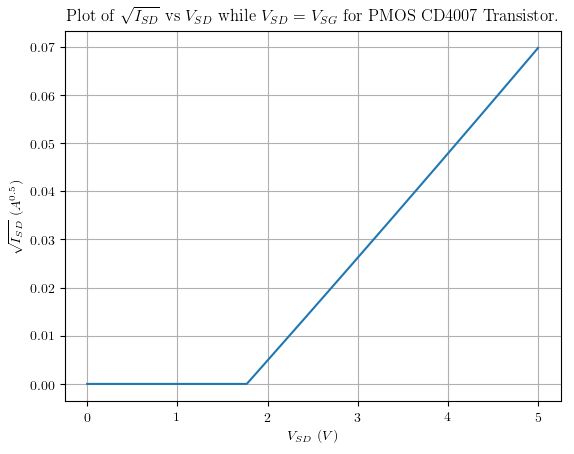
\includegraphics[width = 0.7\textwidth]{figures/part_1_psqrt.png}
        \caption{The graph of $\sqrt{I_{SD}}$ vs $V_{SD}$ for the PMOS
        transistor. It can be seen from the graph that the cut-in
        voltage is the corner at $V_{SD} = 1.40V$ or $V_T = -1.40V$.}
        \label{fig:part_1d_p}
    \end{figure}


    \section{An NMOS inverter}
    The NMOS inverter circuit is shown below in figure
    \ref{fig:inverter_circuit}.
    \begin{figure}[H]
        \centering
        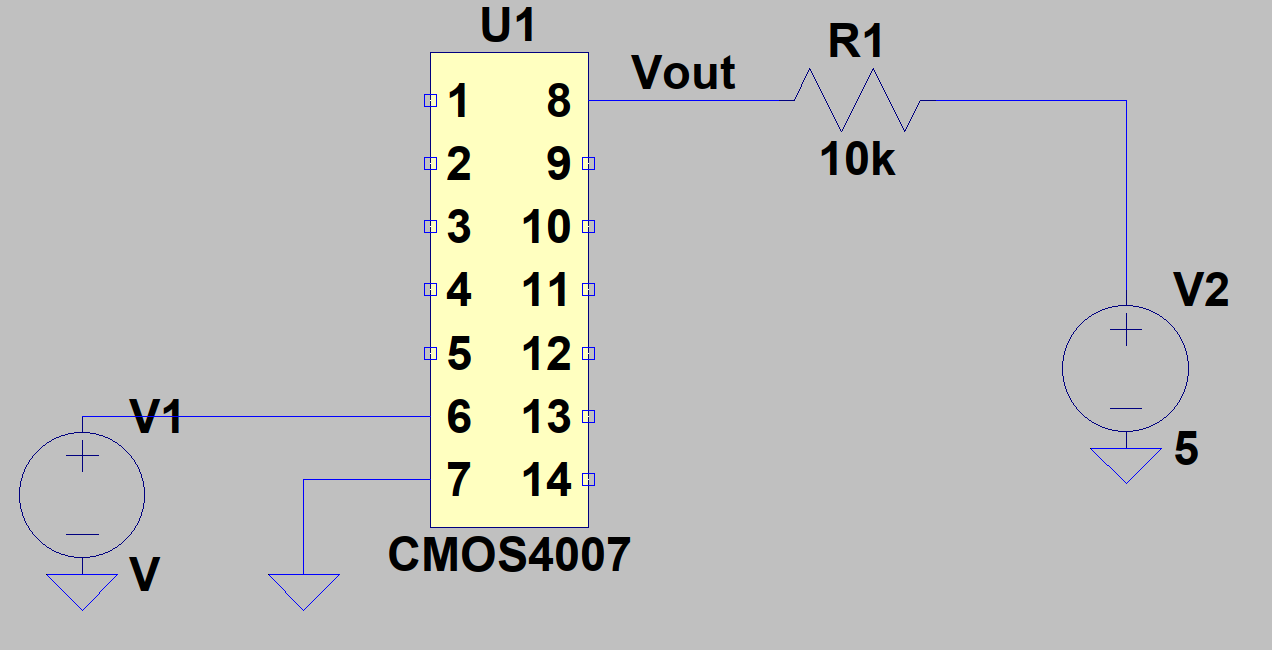
\includegraphics[width=0.7\textwidth]{figures/inverter_circuit.png}
        \caption{The inverter circuit designed in LT Spice}
        \label{fig:inverter_circuit}
    \end{figure}
    The graph of the voltage transfer characteristics for the above
    circuit is then shown in figure \ref{fig:invert_graph}.
    \begin{figure}[H]
        \centering
        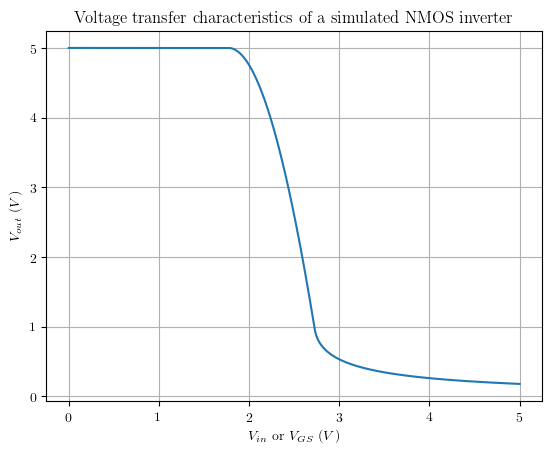
\includegraphics[width=0.7\textwidth]{figures/part_2_invert.png}
        \caption{The graph of the voltage transfer characteristics of
        the NMOS inverter circuit.}
        \label{fig:invert_graph}
    \end{figure}

    \section{Comparison of Data to Real Transistor Devices}
    The nMOS and pMOS iv curves of the real transistor are shown below
    in figures \ref{fig:real_n} and \ref{fig:real_p} respectively.
    \begin{figure}[H]
        \centering
        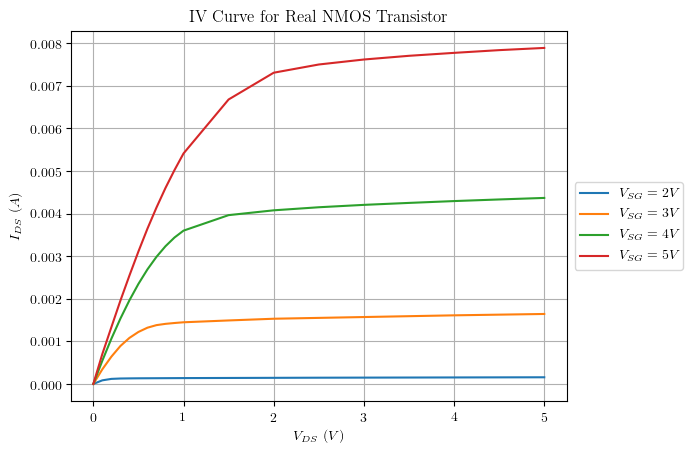
\includegraphics[width=0.7\textwidth]{figures/part_3_nmos.png}
        \caption{The graph of the iv characteristics for the real NMOS
        transistor.}
        \label{fig:real_n}
    \end{figure}
    \begin{figure}[H]
        \centering
        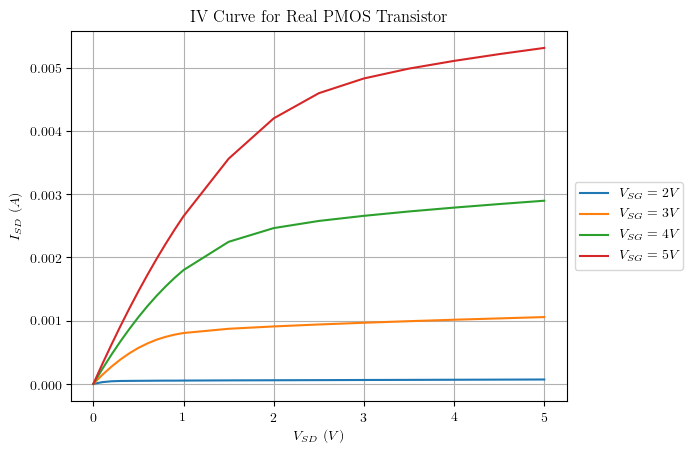
\includegraphics[width=0.7\textwidth]{figures/part_3_pmos.png}
        \caption{The graph of the iv characteristics for the real PMOS
        transistor.}
        \label{fig:real_p}
    \end{figure}
    \subsection{Calculation of parameters of the real transistors}
    \label{sec:real_sol}
    Using the same method from section \ref{sec:nmos_sol}, the following
    iv curves with the cubic approximation are obtained.
    \begin{figure}
        \centering
        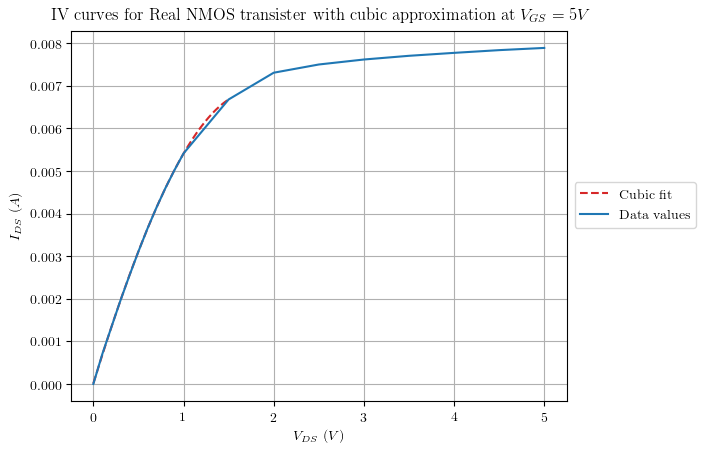
\includegraphics[width=0.5\textwidth]{figures/part_3_ncube.png}
        \caption{The nMOS cubic approximation with the iv curve at
            $V_{GS}= 5V$. The approximation is a very close fit to the
        line.}
    \end{figure}
    \begin{figure}
        \centering
        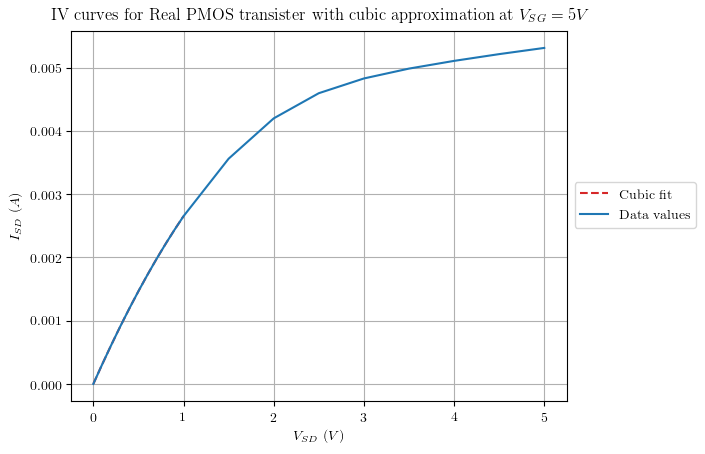
\includegraphics[width=0.5\textwidth]{figures/part_3_pcube.png}
        \caption{The pMOS cubic approximation with the iv curve at
            $V_{SG}= 5V$. The approximation is a very close fit to the
        line.}
    \end{figure}
    Using the script from Appendix \ref{sec:code} we can obtain that for
    the nMOS
    \begin{align*}
        k_n &= 4.236 mA/V^2\\
        \lambda &= 0.137 V^{-1}\\
        V_T &= 3.4V\\
    \end{align*}
    and for the pMOS
    \begin{align*}
        k_n &= 1.149 mA/V^2\\
        \lambda &= 0.0064 V^{-1}\\
        V_T &= -2.2V\\
    \end{align*}
    Clearly these values are very different from the values obtained in
    part 1. The reason for these differences in values from the
    theoretical values determined in LT spice could be do to a number of
    reasons. The largest reasons for the differences will be that LT
    spice assumes an ideal system. The components in LT spice act
    according to the equations used to model them. However the actual
    components in the real world won't exactly follow the equations we
    have developed to model the devices. For example all wires in LT
    spice are assumed to be ideal conductors with no resistance,
    inductance or capacitance, where as in the real world all conductors
    will have all 3 of these properties that can effect the circuit
    operation. Another major consideration is temperature; LT spice will
    assume the temperature of the devices stays constant throughout
    operation however in the real world as a device is used and current
    flows through it power will be dissipated as heat. As the
    temperature of a semiconductor effects conductivity as the
    temperature changes the iv characteristics will change. All of the
    above discussed reasons could have lead to the discrepancies in
    values between the LT SPICE and real circuit data.

    \subsection{The alternative method for calculating Threshold
    Voltage}
    Similarly to with the LT spice simulation, the threshold voltages of
    the real nMOS and pMOS transistors was calculated by tying the
    $V_{GS} = V_{DS}$ and $V_{SG} = V_{SD}$ respectively. The graphs of
    these experiments are shown below.
    \begin{figure}[H]
        \centering
        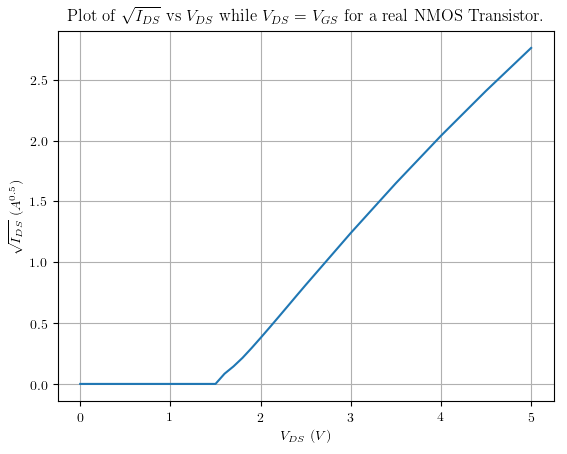
\includegraphics[width=0.7\textwidth]{figures/part_3_nsqrt.png}
        \caption{The graph of $\sqrt{I_{DS}}$ vs $V_{DS}$ for the real
        nMOS transistor. From it we can see that $V_T \approx 1.6V$.}
    \end{figure}
    \begin{figure}[H]
        \centering
        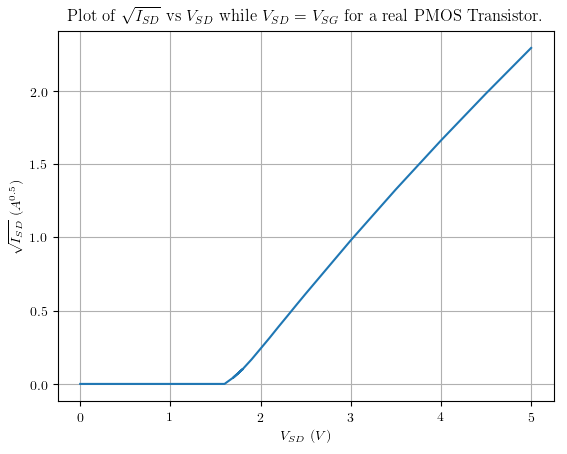
\includegraphics[width=0.7\textwidth]{figures/part_3_psqrt.png}
        \caption{The graph of $\sqrt{I_{SD}}$ vs $V_{SD}$ for the real
        pMOS transistor. From it we can see that $V_T \approx -1.7V$.}
    \end{figure}
    Clearly there is discrepancy between the values calculated for the
    real transistors here as opposed to in section \ref{sec:real_sol}
    and from part 1c however these values are much closer to the ones
    from the simulated transistors then the other real transistor data.
    As seen in sections \ref{sec:sim_sol1} and \ref{sec:sim_sol2} the
    two methods can produce very similar and accurate results. However
    the second method is computationally significantly easier and can
    even be done to some extent in experiment. Being able to do this for
    the actual transistor device is more useful then the simulated as
    the simulated transistor $V_T$ is stated in the library file for LT
    spice, and the value could very slightly between real transistors
    purchased and the theoretical simulated values as seen in these
    experiments. For this reason, it would be best to use the second
    method with a real transistor to find the threshold voltage for when
    building a circuit.

    \subsection{NMOS inverter with a real transistor}
    The real transistor inverter voltage transfer curve is shown below.
    \begin{figure}
        \centering
        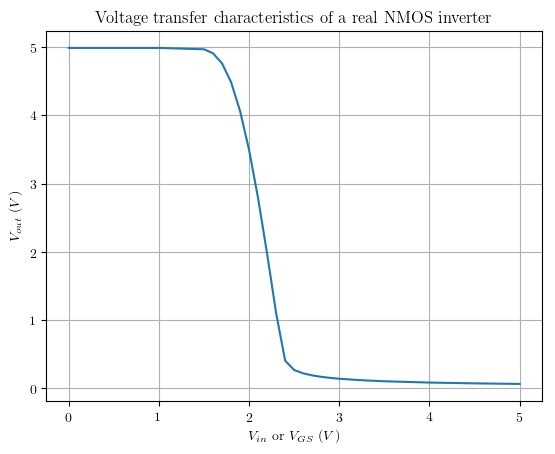
\includegraphics[width=0.7\textwidth]{figures/part_3_invert.png}
        \caption{The voltage transfer characteristics of a real NMOS
        inverter circuit}
        \label{fig:real_inv}
    \end{figure}
    There is some minor discrepancies between the real inverter voltage
    curve and the simulated curve in figures \ref{fig:real_inv} and
    \ref{fig:invert_graph} respectively. The major differences have to
    do with where some of the voltages occur between the two graphs. For
    example $V_{IL}$ is greater than 2V for the simulated graph and less
    than 2V for the real curve. The reasons for this are in part due to
    the difference in threshold voltage between the two transistors; The
    real FET has a $V_T\approx 1.6V$ and the simulated FET is
    $V_T=1.77V$. The lower threshold voltage of the real fet caused the
    inverter to trigger earlier then the simulated FET. The $V_{OL}$ is
    also significantly closer to 0V for the real transistor then the
    simulated one. This and most of the other effects are probably due
    to similar reasons for the discrepancy in IV curves between the
    simulation and real data being that the simulation is a much more
    ideal situation then the actual data in the lab where non ideal
    components must be used.

    \section{Conclusion}
    Even with the differences in the LT Spice simulation software and
    the real data provided, the use of LT Spice is still extremely
    valuable in circuit analysis and design. It allows us to get see how
    a circuit will respond without having to either do the full
    calculations to solve the math, or buy the components and in some
    cases PCBs to properly test our circuit. This can save both time and
    money making it and other simulators like it a very useful tool for
    circuit design and analysis. As with all simulations the differences
    between the theoretical and real world must be taken into account
    but should normally not be too drastic to make large differences to
    the outcome.

    \appendix
    \section*{Appendicies}
    \section{Raw Data for recorded in experiments}\label{sec:data}
    \subsection{Part 1A}
    \subsubsection{$V_{GS} = 2V$}
    \lstinputlisting[style=data]{part_1a/V_GS2.txt}
    \subsubsection{$V_{GS} = 3V$}
    \lstinputlisting[style=data]{part_1a/V_GS3.txt}
    \subsubsection{$V_{GS} = 4V$}
    \lstinputlisting[style=data]{part_1a/V_GS4.txt}
    \subsubsection{$V_{GS} = 5V$}
    \lstinputlisting[style=data]{part_1a/V_GS5.txt}
    \subsection{Part 1B}
    \subsubsection{$V_{SG} = 2V$}
    \lstinputlisting[style=data]{part_1b/V_SG2.txt}
    \subsubsection{$V_{SG} = 3V$}
    \lstinputlisting[style=data]{part_1b/V_SG3.txt}
    \subsubsection{$V_{SG} = 4V$}
    \lstinputlisting[style=data]{part_1b/V_SG4.txt}
    \subsubsection{$V_{SG} = 5V$}
    \lstinputlisting[style=data]{part_1b/V_SG5.txt}
    % \subsection{Part 1D}
    % \subsubsection{nMOS}
    % \lstinputlisting[style=data]{part_1d_nmos.txt}
    % \subsubsection{pMOS}
    % \lstinputlisting[style=data]{part_1d_pmos.txt}

    \section{Python Script for Data Calculation and
    Graphing}\label{sec:code}
    \pythonexternal{lab1.py}

\end{document}
